\section{Introduction to Distributed Data Fusion}

\begin{frame}
	\frametitle{Multi-Agent Multi-Object Tracking (MAMOT)}
	\framesubtitle{A brief overview}
	
	\begin{columns}
		\column{.7\textwidth}
		\centering
		
		\begin{block}{Object Tracking}
			Detect objects and follow their trajectories
		\end{block}
		
		\begin{block}{MAMOT}
			A team of agents estimate the object trajectories using sensors with a limited field-of-view
		\end{block}
		
		\begin{itemize}
			\item distributed environment (network connected agents)
			\item best-effort communication channel
		\end{itemize}
		
		\column{.28\textwidth}
		\centering
		
		\begin{tikzpicture}
			\node at (0,0) [draw=black,ultra thick,inner sep=0pt]  {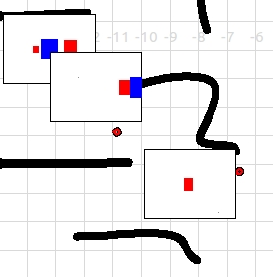
\includegraphics[width=3cm]{Figures/Player.png}};
		\end{tikzpicture}
	\end{columns}
\end{frame}

\begin{frame}
	\frametitle{Issues on DDF}
	\framesubtitle{The Data Association problem}
	
	\begin{columns}[T]
		\column{.55\textwidth}
		
		\begin{itemize}
			\only<1>{\item In MAMOT, the pool of gathered parameters are used to compute the global estimation}
			\only<1>{\item Using a Particle Filter, one of the main problem that arises is how to avoid poor estimation
						   quality}
			\only<1>{\vspace{3.42cm}}
			\only<2->{\item The weight of particles is evaluated using the received parameters}
			\only<3->{\vspace{1.5cm}\item[1] Using all parameters influences the whole distribution}
			\only<4-5>{\vspace{1.1cm}}
			\only<6>{\vspace{0.9cm}}
			\only<4>{\item[2] We can assign better weights by use clustering before weighting}
			\only<5>{\item[2] The parameters are associated to the clusters}
			\only<6>{\item[2] The weights of particles in a cluster is given by the parameters associated to it}
		\end{itemize}
		
		\column{.45\textwidth}
		\centering
		
		\begin{tikzpicture}
			\only<1>
			{
				\node at (0,0) [draw=white,thick,inner sep=0pt]  {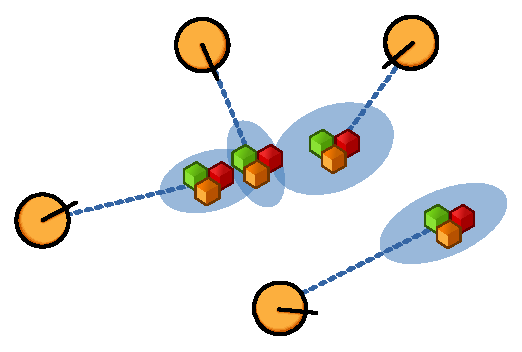
\includegraphics[width=5cm]{Figures/MamotDDF.pdf}};
			}
			\only<2->
			{
				\node at (-1.3,0) [draw=white,thick,inner sep=0pt]  {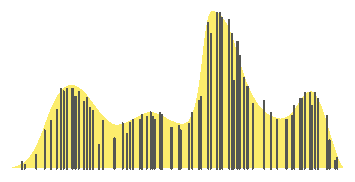
\includegraphics[width=2.5cm]{Figures/Issue0.pdf}};
				\node at (1.3,0) [draw=white,thick,inner sep=0pt]  {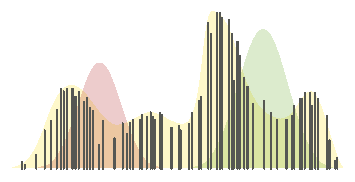
\includegraphics[width=2.5cm]{Figures/Issue0Bis.pdf}};
				\node at (0,-1) [inner sep=0pt]  {
\includegraphics[width=5cm]{Figures/Parentheses.pdf}};
				\node at (0,-2.5) [draw=white,thick,inner sep=0pt]  {
\includegraphics[width=4cm]{Figures/IssueBlank.pdf}};
				\node at (0,-4.8) [draw=white,thick,inner sep=0pt]  {
\includegraphics[width=4cm]{Figures/IssueBlank.pdf}};
			}
			\only<3->
			{
				\node at (0,-2.5) [draw=white,thick,inner sep=0pt]  {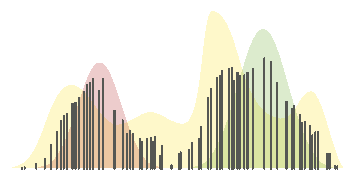
\includegraphics[width=4cm]{Figures/Issue1.pdf}};
				\node at (0,-4.8) [draw=white,thick,inner sep=0pt]  {
\includegraphics[width=4cm]{Figures/IssueBlank.pdf}};
			}
			\only<4>
			{
				\node at (0,-4.8) [draw=white,thick,inner sep=0pt]  {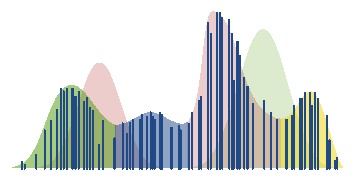
\includegraphics[width=4cm]{Figures/Issue2.pdf}};
			}
			\only<5>
			{
				\node at (0,-4.8) [draw=white,thick,inner sep=0pt]  {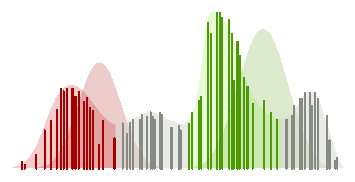
\includegraphics[width=4cm]{Figures/Issue2Bis.pdf}};
			}
			\only<6>
			{
				\node at (0,-4.8) [draw=white,thick,inner sep=0pt]  {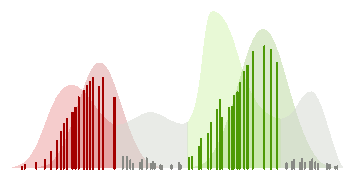
\includegraphics[width=4cm]{Figures/Issue2Ter.pdf}};
			}
		\end{tikzpicture}
	\end{columns}
\end{frame}
